\chapter[La materia oscura]{Bertin-La materia oscura}

Prima di scendere nei particolari della trattazione della materia oscura, dobbiamo specificare in che campo ci stiamo muovendo: parleremo infatti di qualcosa della quale è stata dimostrata l'esistenza, ma di cui non abbiamo ancora avuto contatto in prima persona, e dunque non sappiamo di cosa stiamo effettivamente parlando.

\section{La scoperta delle galassie}

Per spiegare cosa rappresentino le galassie nel mondo astrofisico, possiamo utilizzare la seguente frase:
\begin{center}
\emph{What are the galaxyes? No one knew before $1900$.\\
Very few people knew in $1920$. All astronomers knew after $1924$.\\}
\end{center}
\begin{center}
\textit{(Allan Sandage, The Hubble Atlas of Galaxies, $1961$)\\}
\end{center}
La scoperta delle galassie è storicamente individuata nell'anno $1924$; in effetti, prima di quell'anno nei cataloghi di oggetti celesti erano presenti alcune galassie, ma erano segnalate come oggetti estesi, come nel caso di M1, M16, M31, M51, M81 e M101 nel catalogo di Messier; questo è dovuto al fatto che a quei tempi non si sapeva se tali oggetti fossero stelle deboli ma molto vicine a noi o stelle molto luminose ma lontanissime.\\
Nel $1924$ l'astronomo americano Hubble misurò la distanza di alcune di queste ``nebulose'' vicine, come per esempio M31 (galassia di Andromeda), e scoprì che tali oggetti sono distanti milioni di anni luce e che oggetti morfologicamente simili (ad esempio M1) possono essere distanti addirittura miliardi di anni luce.\\

Prima della scoperta di Hubble, a cavallo degli anni $'20$, la caratterizzazione di questi oggetti estesi era già oggetto di una controversia scientifica; possiamo distinguere due ``scuole'', entrambe con tesi e motivazioni scientificamente ragionevoli:
\begin{itemize}
\item Tali oggetti sono molto vicini a noi,e dunque si tratta di stelle molto deboli; tale fazione era ``capeggiata'' da Shapley
\item Tali oggetti sono lontani da noi,e dunque sono luminosissimi; tale fazione era ``capeggiata'' da Curtis
\end{itemize}
Come già sappiamo, le misure di Hubble daranno ragione a questi ultimi e apriranno le porte ad un nuovo tipo di oggetto celeste, le galassie; è giusto però sottolineare ancora una volta che le ragioni dei primi non sono ``campate per aria'' e irragionevoli, nonostante poi la tesi da loro sostenuta si sia rivelata errata.

Tornando alle misure compiute da Hubble, vediamo che venne osservata un'altra particolarità all'interno di queste ``nebulose'': infatti Hubble notò che c'erano delle stelle che variavano in luminosità con un periodo ben preciso; tali stelle sono attualmente note con il nome di Cefeidi variabili. Su alcune di esse venne compiuta un analisi temporale che permise di ricavarne il periodo; alcuni esempi sono riportati nei grafici qua sotto, dove in realtà sono stati raccolti dati a periodi diversi.

\begin{figure}[!h]
\centering
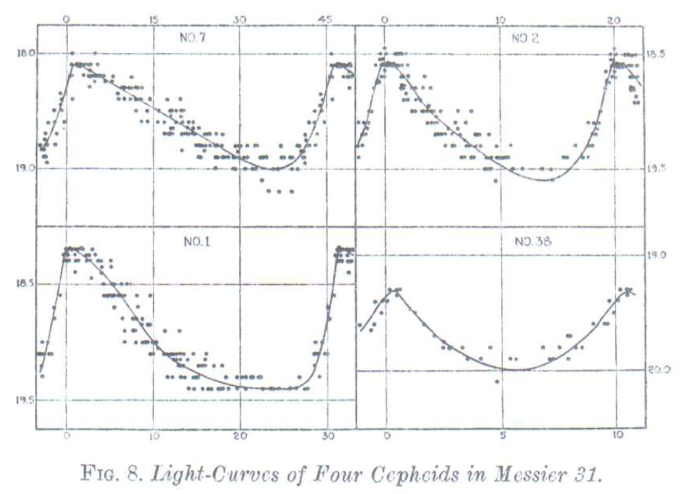
\includegraphics[width=0.8\textwidth]{Img/bertin_18.png}
\end{figure}

Noriamo che per le stelle più luminose il periodo è più lungo, mentre per quelle meno luminose è più breve; oltretutto, Hubble ricavò che esistono due tipi di Cefeidi, fatto che porta ad un errata misura delle dimensioni della stella. Supponiamo di avere una sola relazione in gioco, cioè che la luminosità apparente $L_ {app} \sim \frac{L}{R^2}$: dato che la luminosità è legata al periodo (in prima approssimazione, $L \propto \log T$) del quale è possibile ricavare una misura, possiamo dedurre la distanza $R$ della stella; in questo modo Hubble misurò distanze molto grandi ma errate di un fattore $2$: per esempio ricavò che la distanza di M31 era di $300 \, kpc$, mentre attualmente il valore riconosciuto è $770 \, kpc$.
\\
Una volta che conosciamo la distanza di una stella, come possiamo utilizzare tale dato per dedurre proprietà intriseche della stella? Dato che siamo in grado di misurarne la dimensione angolare, possiamo ricavare una stima del diametro $L \sim 1 \div 100 \, kpc$, anche se tale stima è affetta da errore poichè è difficile definire i contorni di una galassia (solitamente si considera la zona da cui proviene il $50 \%$ della luminosità); a questo punto, effettuando una proporzione con il Sole, possiamo stimare la massa di una galassia che è nell'ordine di $10^9 \div 10^{12} \, M_{\odot}$; possiamo infine ricavare il tempo dinamico $T_{din} \sim 10^8 \div 10^9 \, yr$, dove $1 yr \sim \pi \cdot 10^7 \, s$.
\\
\begin{minipage}{.35\textwidth}
\centering
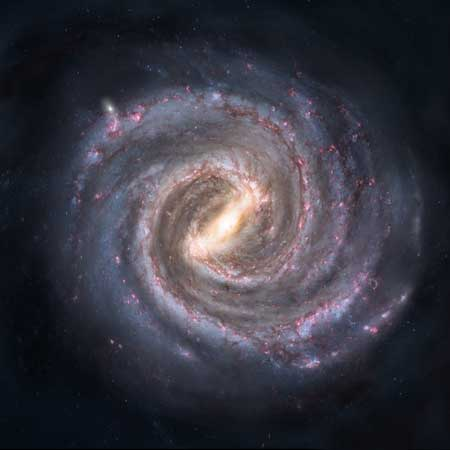
\includegraphics[width=1\textwidth]{Img/via_lattea.jpg}
\end{minipage}
\begin{minipage}{.65\textwidth}
\textbf{Alcuni dati numerici riguanti la Via Lattea}:
Massa: $M \sim 2 \cdot 10^{11} \, M_{\odot}$\\
La distanza del Sole dal centro della galassia è $R_{\odot} \sim 8 \, kpc$, mentre la velocità con cui ruota è $v_{\odot} \sim 220 \, \frac{km}{s}$, con un periodo di rotazione $T_{\odot} \sim 200 \cdot 10^6 \, yr$\\
La densità è $\Sigma \sim 50 \, M_{\odot}pc^{-2}$, che è circa la densità di un foglio di carta.\\
\end{minipage}

\vspace{0.2cm}

Possiamo inoltre calcolare l'accelerazione radiale del Sole, che vale $A_{r, \odot}= v_{\odot}^2 R_{\odot}^{-1}$. Se invece volessimo stimare l'accelerazione gravitazionale che il disco della galassia opera su una stella che si trova poco fuori dal disco stesso, possiamo ragionare come per una lastra carica elettricamente; ricaviamo allora prima di introdurre il problema $A_z = 2 \pi G \Sigma$.

Quello riportato a di seguito è detto \textbf{tuning fork diagram} per la sua forma che ricorda quella di un diapason; la paternità di tale grafico è attribuita ad Hubble, il quale quasi in contemporanea con le sue misure e osservazioni divise le galassie in tre famiglie in base alla loro forma: abbiamo dunque che le galassie possono essere ellittiche, a spirale e a spirale barrata; in particolare, le galassie a spirale e a spirale barrata si distinguono da quelle ellittiche per la loro forma più schiacciata e per la presenza di un disco di rotazione, e al loro interno sono divise in tre sottocategorie indicate dalle lettere a, b, c. La Via Lattea si trova più o meno a metà fra le galassie di tipo Sb e SBb.

\begin{figure}[!h]
\centering
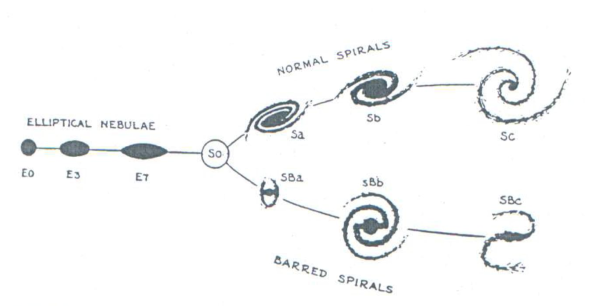
\includegraphics[width=0.8\textwidth]{Img/bertin_20.png}
\end{figure}

\section{Misure di massa}

Finora abbiamo dato un indicazione della massa di molti degli oggetti citati, e potremmo in realtà farlo per tutti gli oggetti celesti; la domanda che ci si pone allora è come faccia l'astronomo a ``pesare'' gli oggetti in cielo, cioè qual'è il procedimento per cui è possibile effettuare misure di massa. Prima di discutere questo punto, però, dobbiamo distinguere fra modello dinamico, cioè il modello con il quale descriviamo il nostro oggetto celeste, e ragionevole aspettazione, cioè quell'insieme di ipotesi su cui l'astronomo si basa e che devono essere adeguatamente giustificate.

L'ipotesi base da cui partiamo è che i fotoni che vediamo sono emessi dalle stelle; infatti la quantità di gas ionizzato all'interno degli altri oggetti (ad esempio il mezzo interstellare, che compone la maggior parte della materia in un gruppo di stelle) è molto poca. Grazie a questo, possiamo dire che la luminosità e la massa della stella osservata sono legate da qualche relazione, e ragionevolmente tale relazione sarà lineare; siccome il Sole è una stella ``normale'', cioè non è una nana bianca o un altra stella particolare, possiamo utilizzarne i valori di massa e luminosità come unità di misura; avremo allora che per una stella con luminosità totale $\L$ possiamo scrivere:
$$\M=\frac{M_{\odot}}{L_{\odot}} \L$$
Un problema irrisolto riguardante la massa delle galassie è quello per cui, nel momento in cui si mette in gioco un modello dinamico, le accelerazioni che si ricavano da tale modello risultano essere significativamente più piccole delle accelerazioni realmente presenti.
\\
\\
Andiamo ora a vedere una misura molto particolare, che ci introdurrà al problema della \textbf{missing mass} (massa mancante), che oggi viene chiamata materia oscura e che ci restituisce accelerazioni compatibili con quelle osservate.

\begin{figure}[!h]
\centering
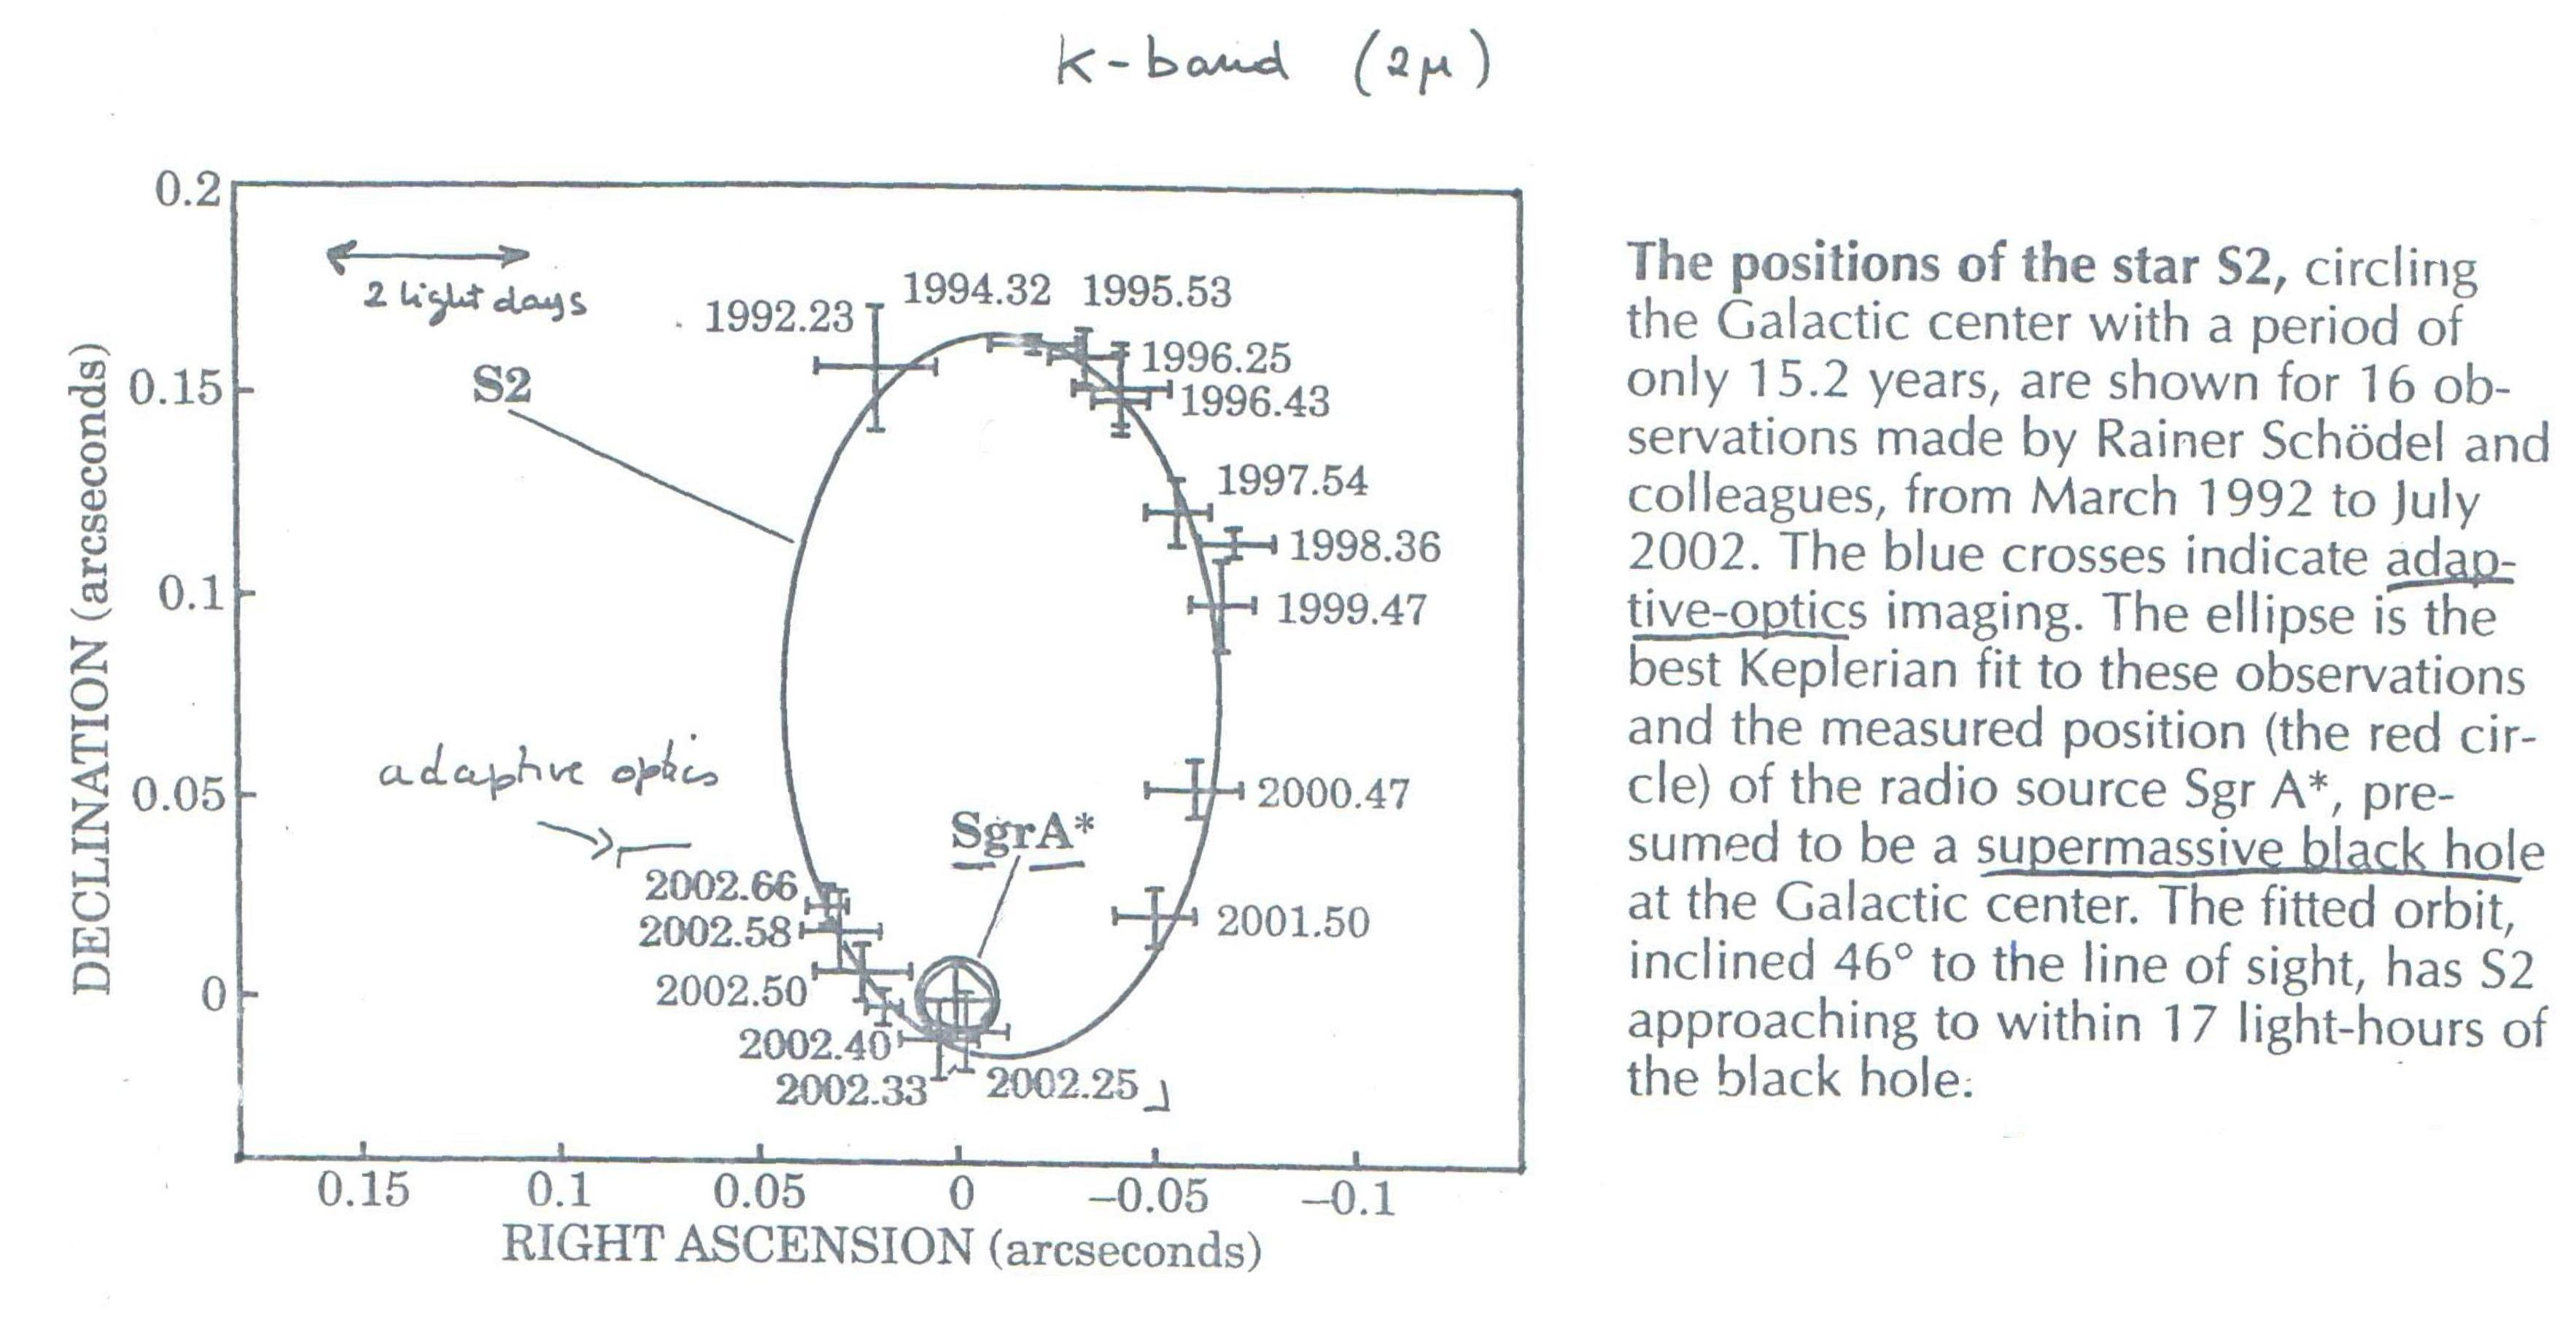
\includegraphics[width=0.85\textwidth]{Img/bertin_21bis.jpg}
\end{figure}

Sugli assi di questo grafico abbiamo la declinazione (la nostra solita $\delta$) e l'ascensione retta (misurata in arcosecondi), i quali sono una coppia di coordinate standard per descrivere la volta celeste; l'origine degli assi viene definita in modo tale che lo zero degli assi stia dove vogliono gli astronomi, e in questo caso essa viene posta  in direzione della costrellazione del Saggittario (SgrA$^*$), dove la Via Lattea si fa più luminosa e più scura perchè siamo guardando verso il centro della nostra galassia ma al contempo la polvere interstellare, come abbiamo già avuto modo di vedere, fa da schermo. Qui interviene l'utilizzo di una particolare banda dello spettro luminoso, la \textbf{banda K} (corrispondente alla lunghezza d'onda di $2 \, \mu m$; la misura consiste nel seguire stella (nel nostro caso, $S2$) rilevandone le posizioni in tempi diversi. %Voce00033, 19:53